% !TEX root = ../thesis.tex

\section{Network Architectures}

In this section, we describe the implementation details of the neural network models we build for social signal prediction. Our method takes the social signals from conversational partners as input and produces the target person's social signals as output. Figure~\ref{fig:inputOutput} shows 3D measurements used for the input and output of our method, where the signals rendered by green and yellow colors are the input, and the social signals rendered by blue color are the output. The output signals include social formation information (position, face orientation, and body orientation), and body motion, and a binary label for the speaking status of the target person. 

In our method, we divide the social signal prediction task into several sub-tasks focusing on predicting a subset of social signals, and the corresponding network architecture for each task is shown in Figure~\ref{fig:architectures}. All of our networks are based on 1D fully convolutional neural networks. In general, our model does not require a fixed window size for the input, but we separate input data into small clips with a fixed size (denoted by $f$) for the efficiency in training. During testing time, our models can be applied to the input of arbitrary length. We use $f=120$, about 4 seconds, for the input window size. The basic architecture follows the work of Holden et al.~\cite{holden2016deep} that demonstrates a compelling result for the mapping between a 2D trajectory and human motions. We modify the network architecture based on the input and output dimensions. 

\subsection{Dimensions of Social Signal Representations}
We describe the dimensions of social signal representations, used for the input and output of our method.

\paragraph{Trajectory (Position + Orientations):} We use a 2D vector for the position and 2D unit vectors for the face orientation and body orientation, defined on the $xz$-plane. Thus the status of an individual at a frame in social formation prediction is represented by a 6-dimensional vector.

\paragraph{Body Gestures:} We follow the body motion representation of the work of Holden et al.~\cite{holden2016deep}, representing a body gesture at a frame as a 73-dimensional vector. This representation is based on the skeletal structure of CMU Mocap dataset~\cite{gross2001cmu} with 21 joints (63 dimensions), along with additional dimensions for a floor point (3 dimensions), velocities for the root movement (3 dimensions relative body translation and orientation), and footstep signals (4 dimensions). We perform a retargeting to convert our 3D motion data from the Panoptic Studio (following the skeleton definition of COCO dataset~\cite{coco-14}) to this CMU Mocap format. For the face signal we use a subpart (initial 5 dimensions) of the facial expression parameters of Adam model~\cite{joo2018,cao2014facewarehouse}, because we found the later dimensions have almost negligible in our reconstruction quality.

\begin{figure}[t]		
	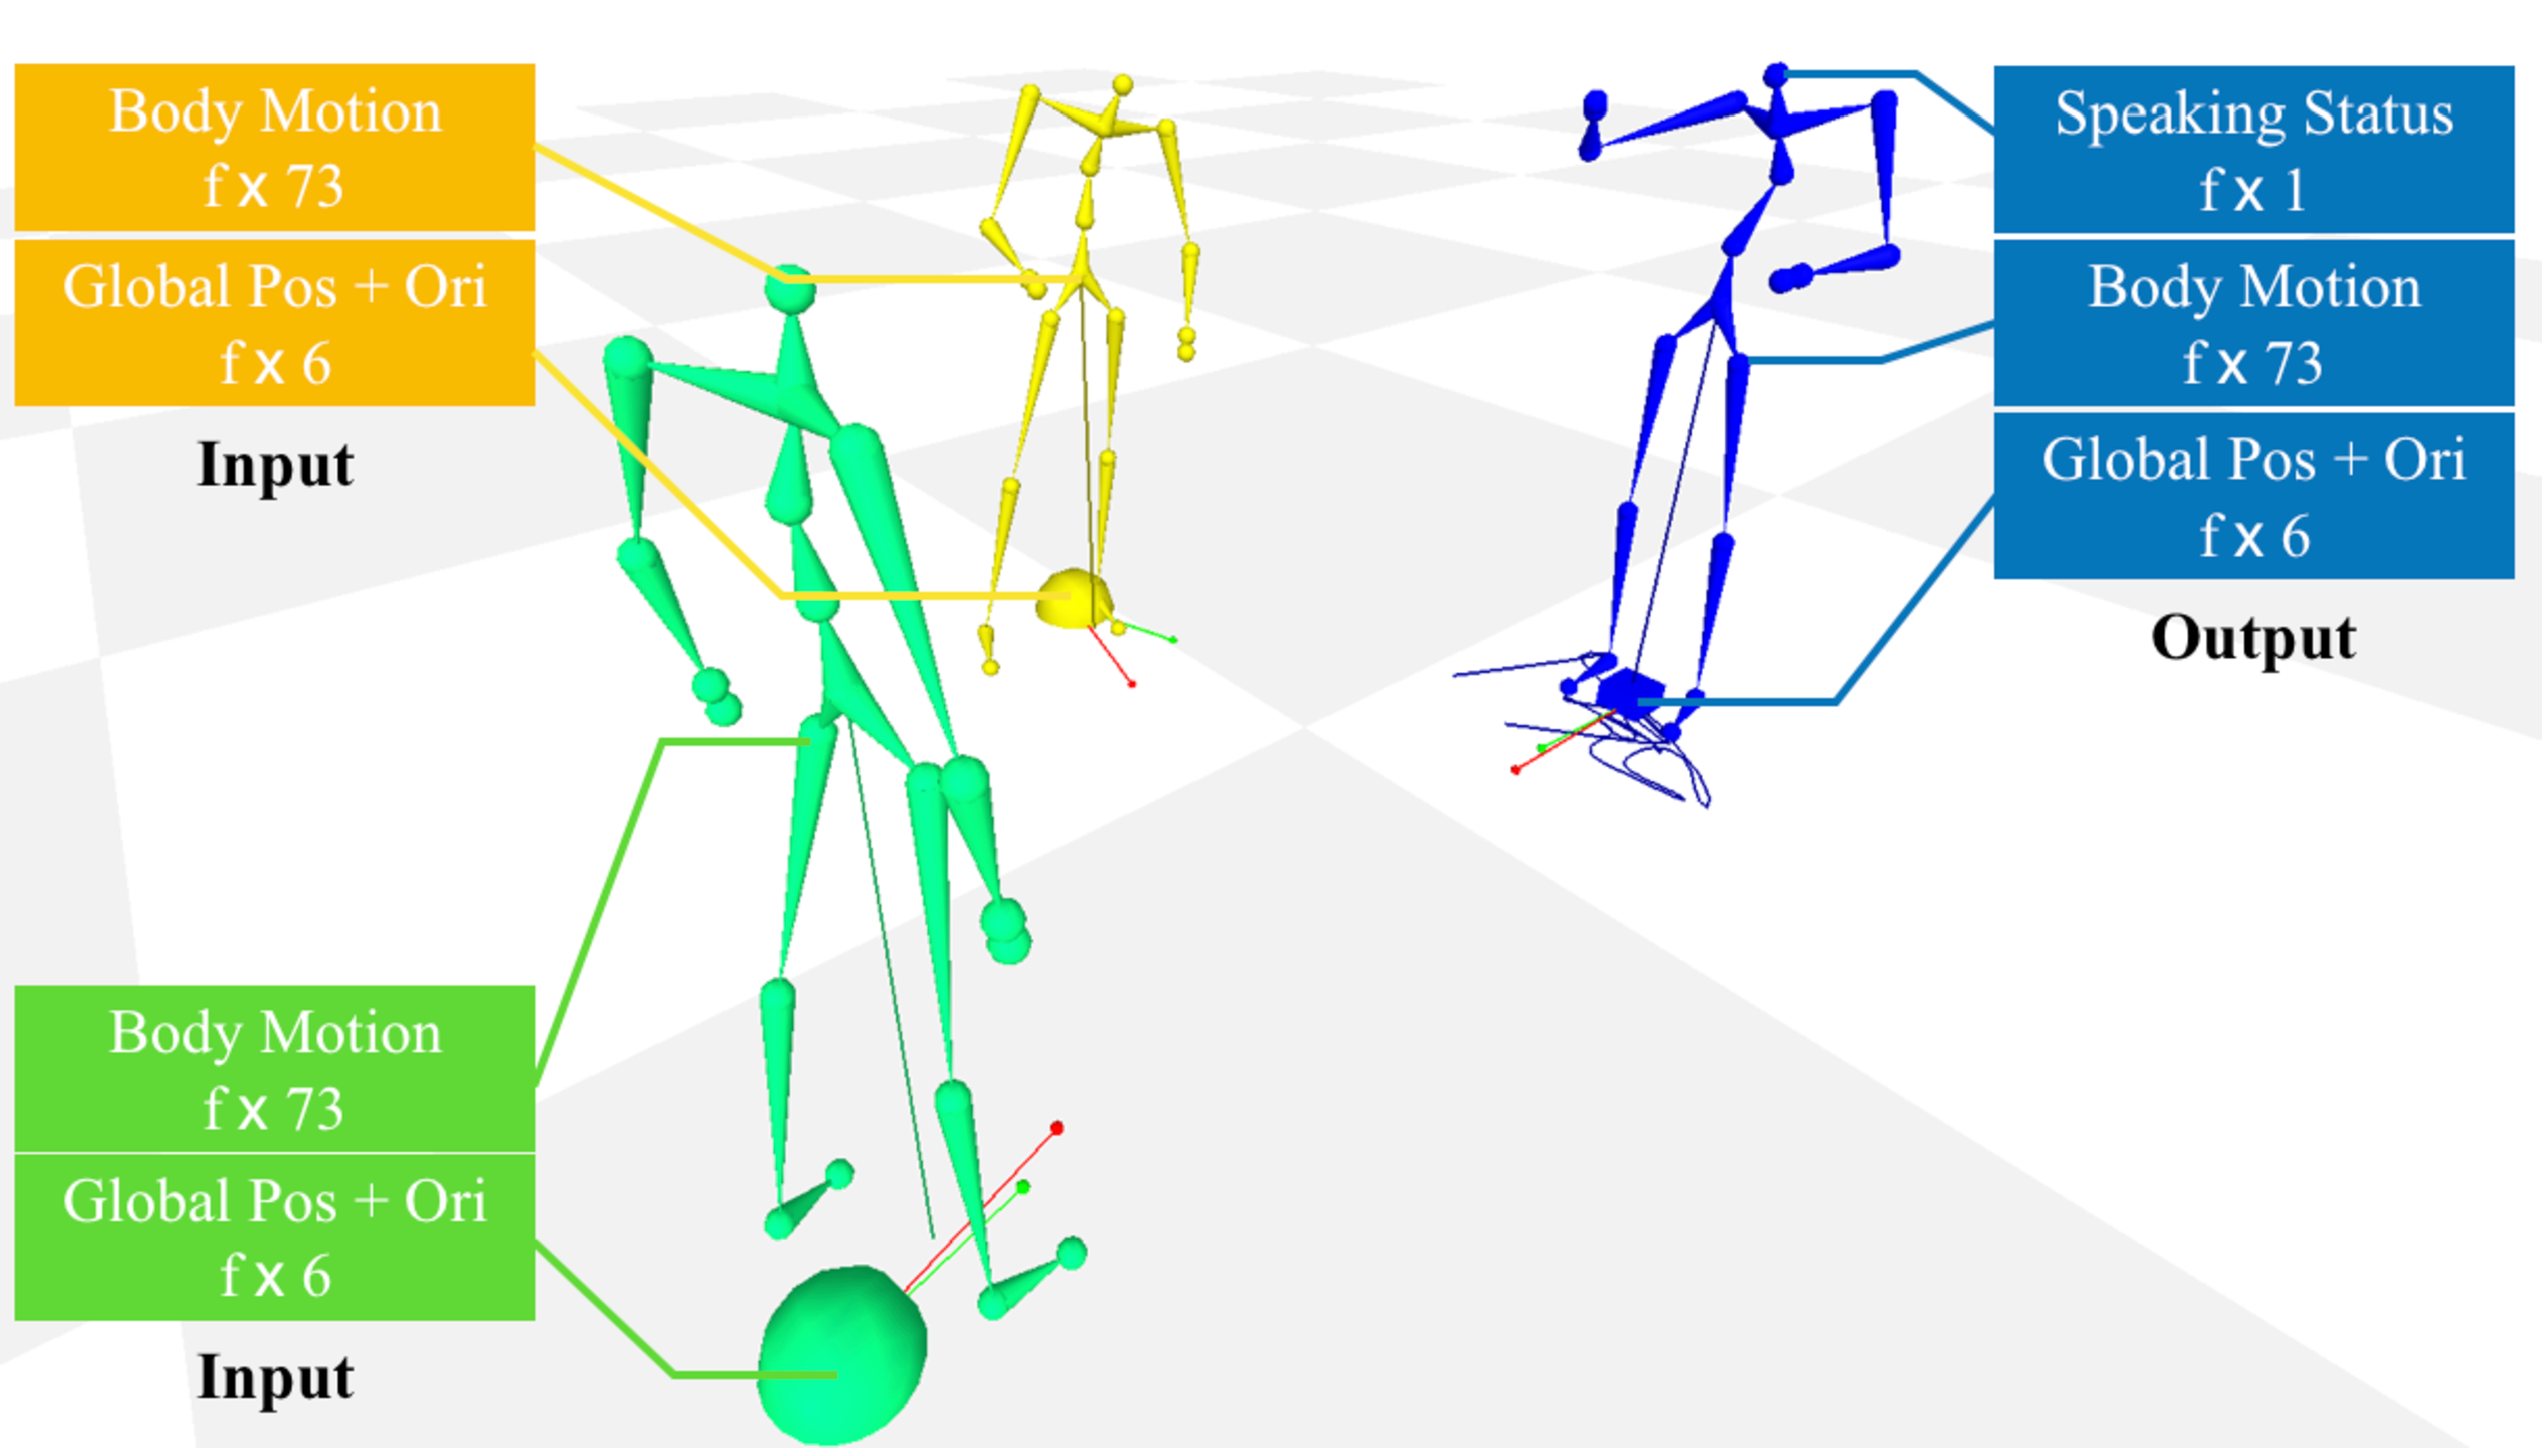
\includegraphics[width=\linewidth]{ssp_fig/Input_output.pdf}
	\caption{The input and output of the Social Signal Prediction task. Our method uses the social signals of conversation partners (green and yellow) as input, and produces the target person's social signals (blue) as output. We consider input and output with an arbitrary length, where the length is denoted as $f$ in this figure. The second dimensions of input and output matrices represent the dimensions of social signals in our representation.}
	\label{fig:inputOutput}
\end{figure}

\begin{figure*}[t]	
	%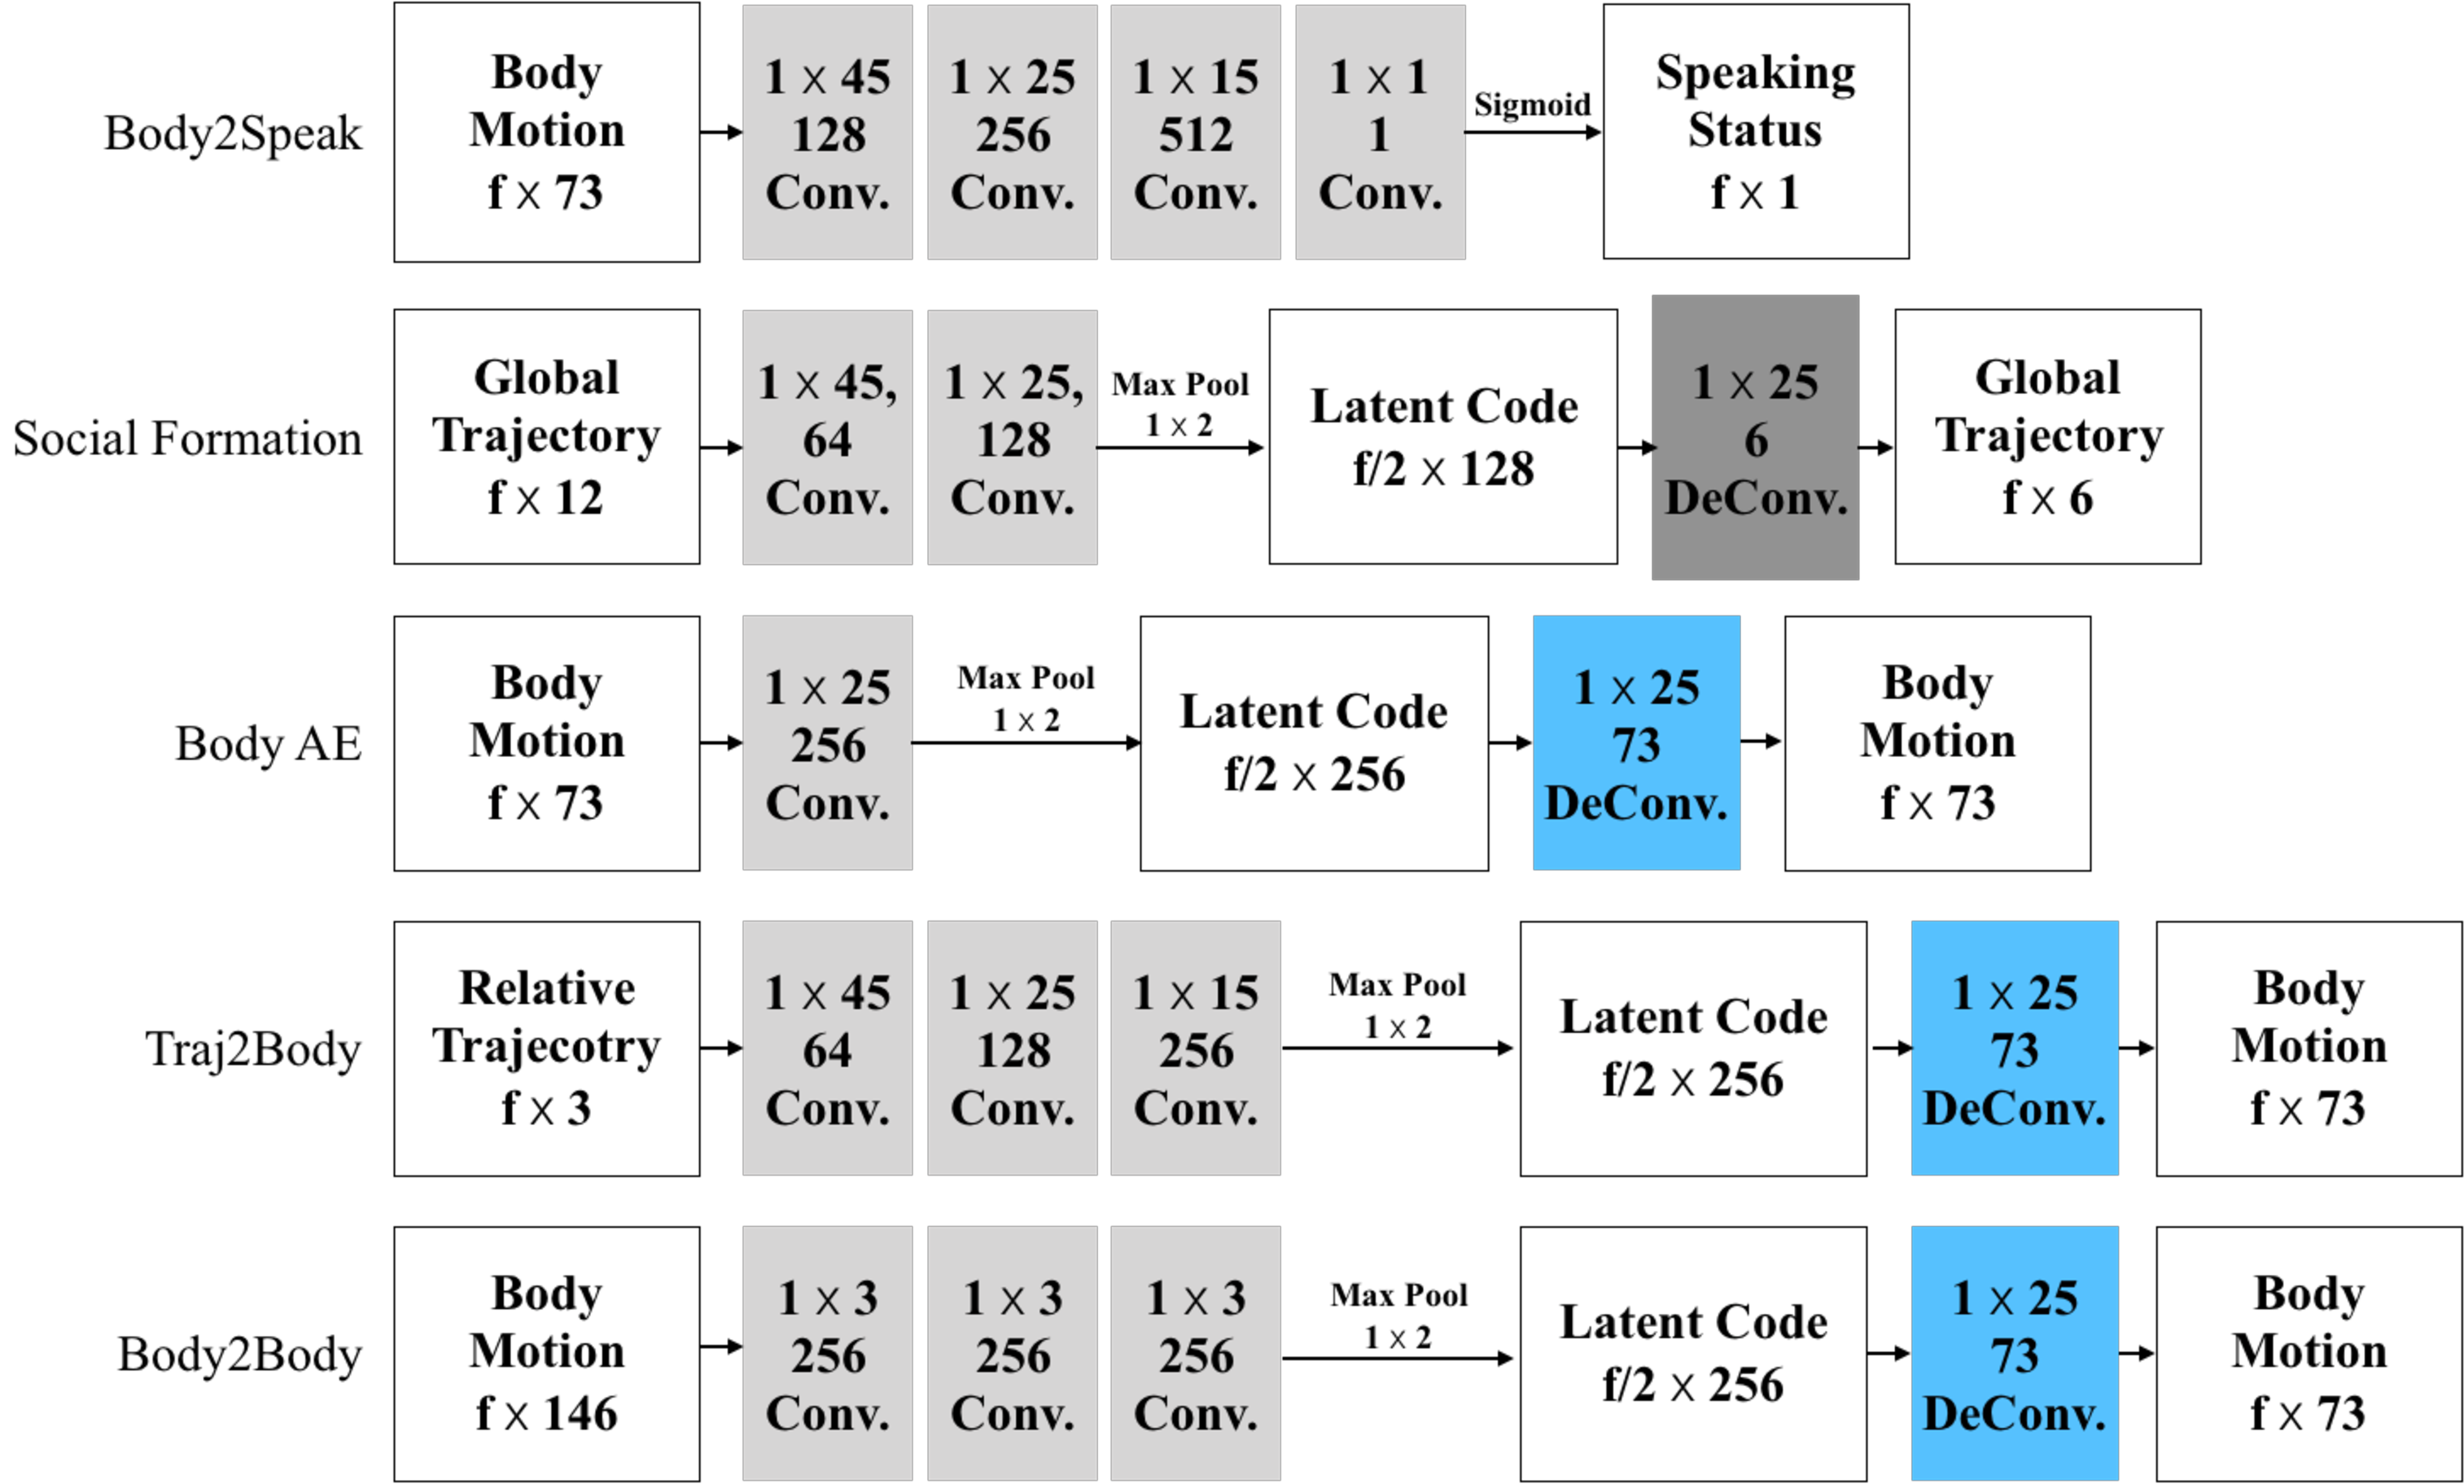
\includegraphics[width=\textwidth]{ssp_fig/networks}
	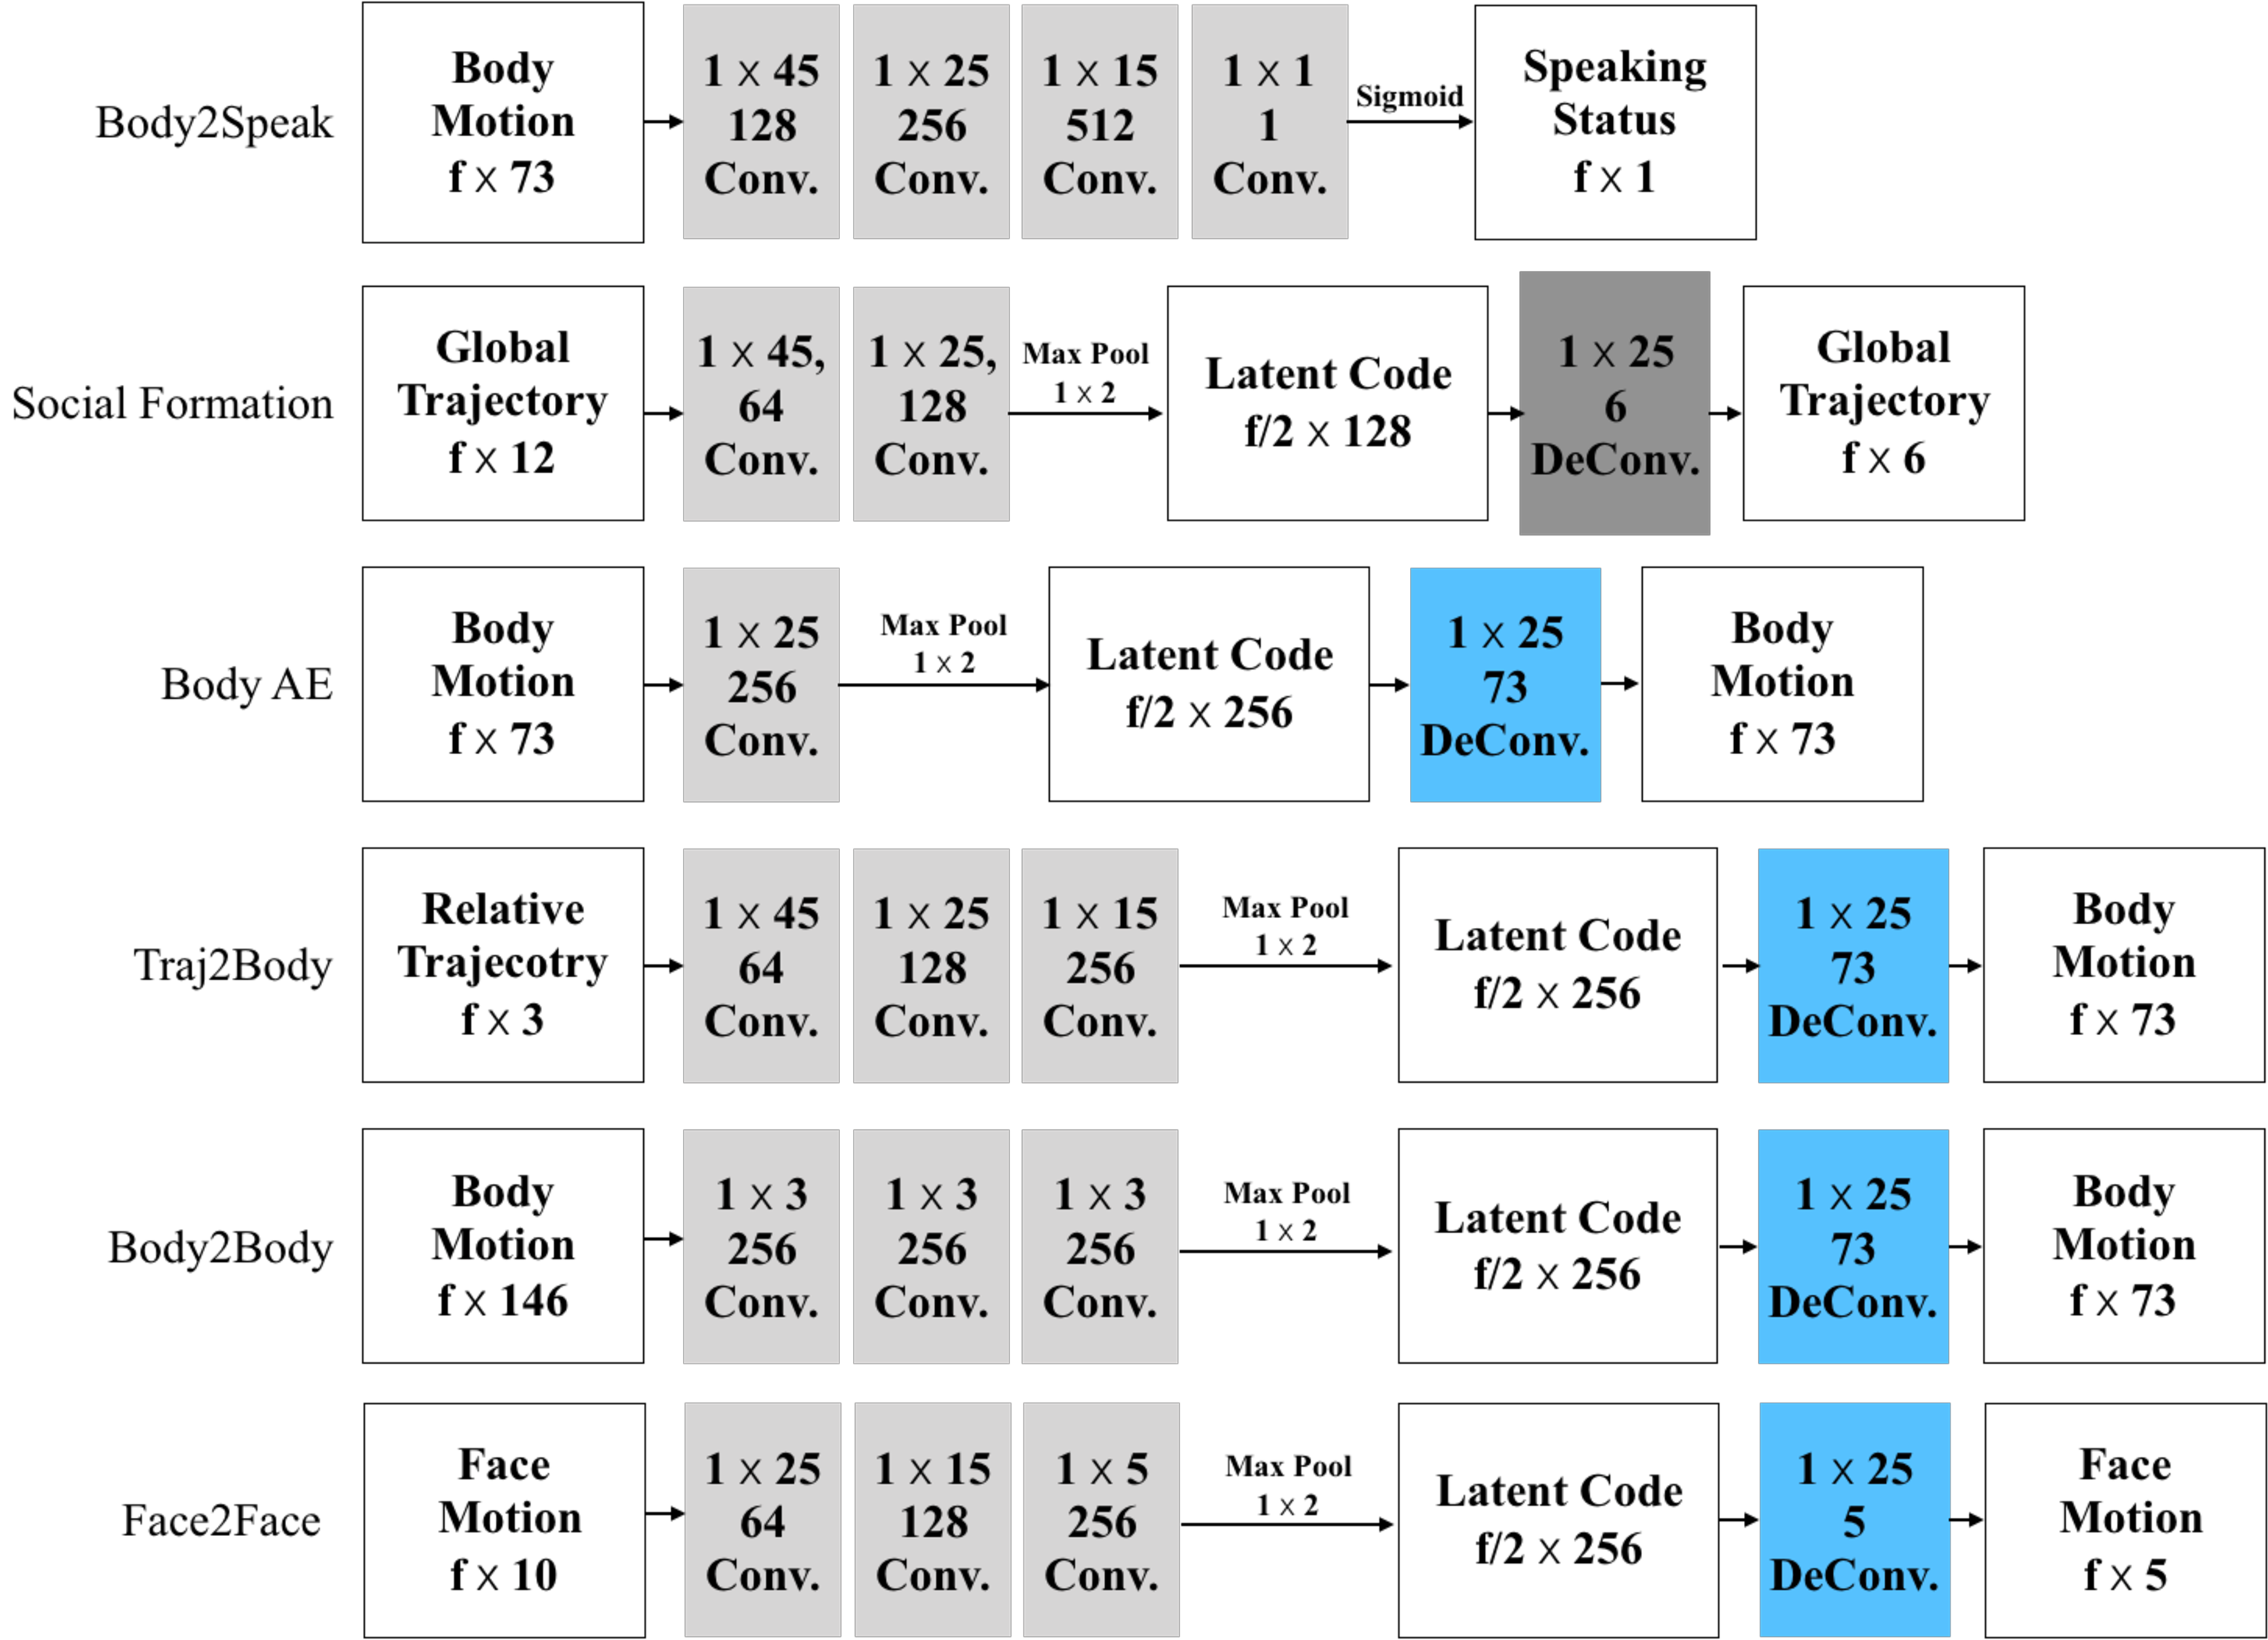
\includegraphics[width=\textwidth]{ssp_fig/networks_face}
	\caption{Network Architectures. We use fully convolutional networks to predict sub-parts of our social signal prediction. We adopts the architecture of Holden et al.~\cite{holden2016deep}, and modify the dimensions and structures based on the input and output dimensions. }
	\label{fig:architectures}
\end{figure*}



\subsection{Predicting Speaking from Body Motion (Body2Speak)}
The input of this network is the body motion of the other seller in the haggling sequence, which is a $f \times 73$ matrix, where $f$ is the number of frames of an input sequence. Here, we ignore the buyer's body motion because often little movement is observed from the buyers.  We use four convolutional layers for the network where the last layer has $1\times1$ convolutions, followed by a sigmoid activation layer. The network architecture is shown in the first row of Figure~\ref{fig:architectures}.


\subsection{Social Formation}
The input of the social formation network is the concatenation of global position and orientation information of the communication partners, represented by a $f \times 12$ matrix.  We use a simple autoencoder structure, as shown in the second row of Figure~\ref{fig:architectures}.

\begin{figure*}[t]	
%	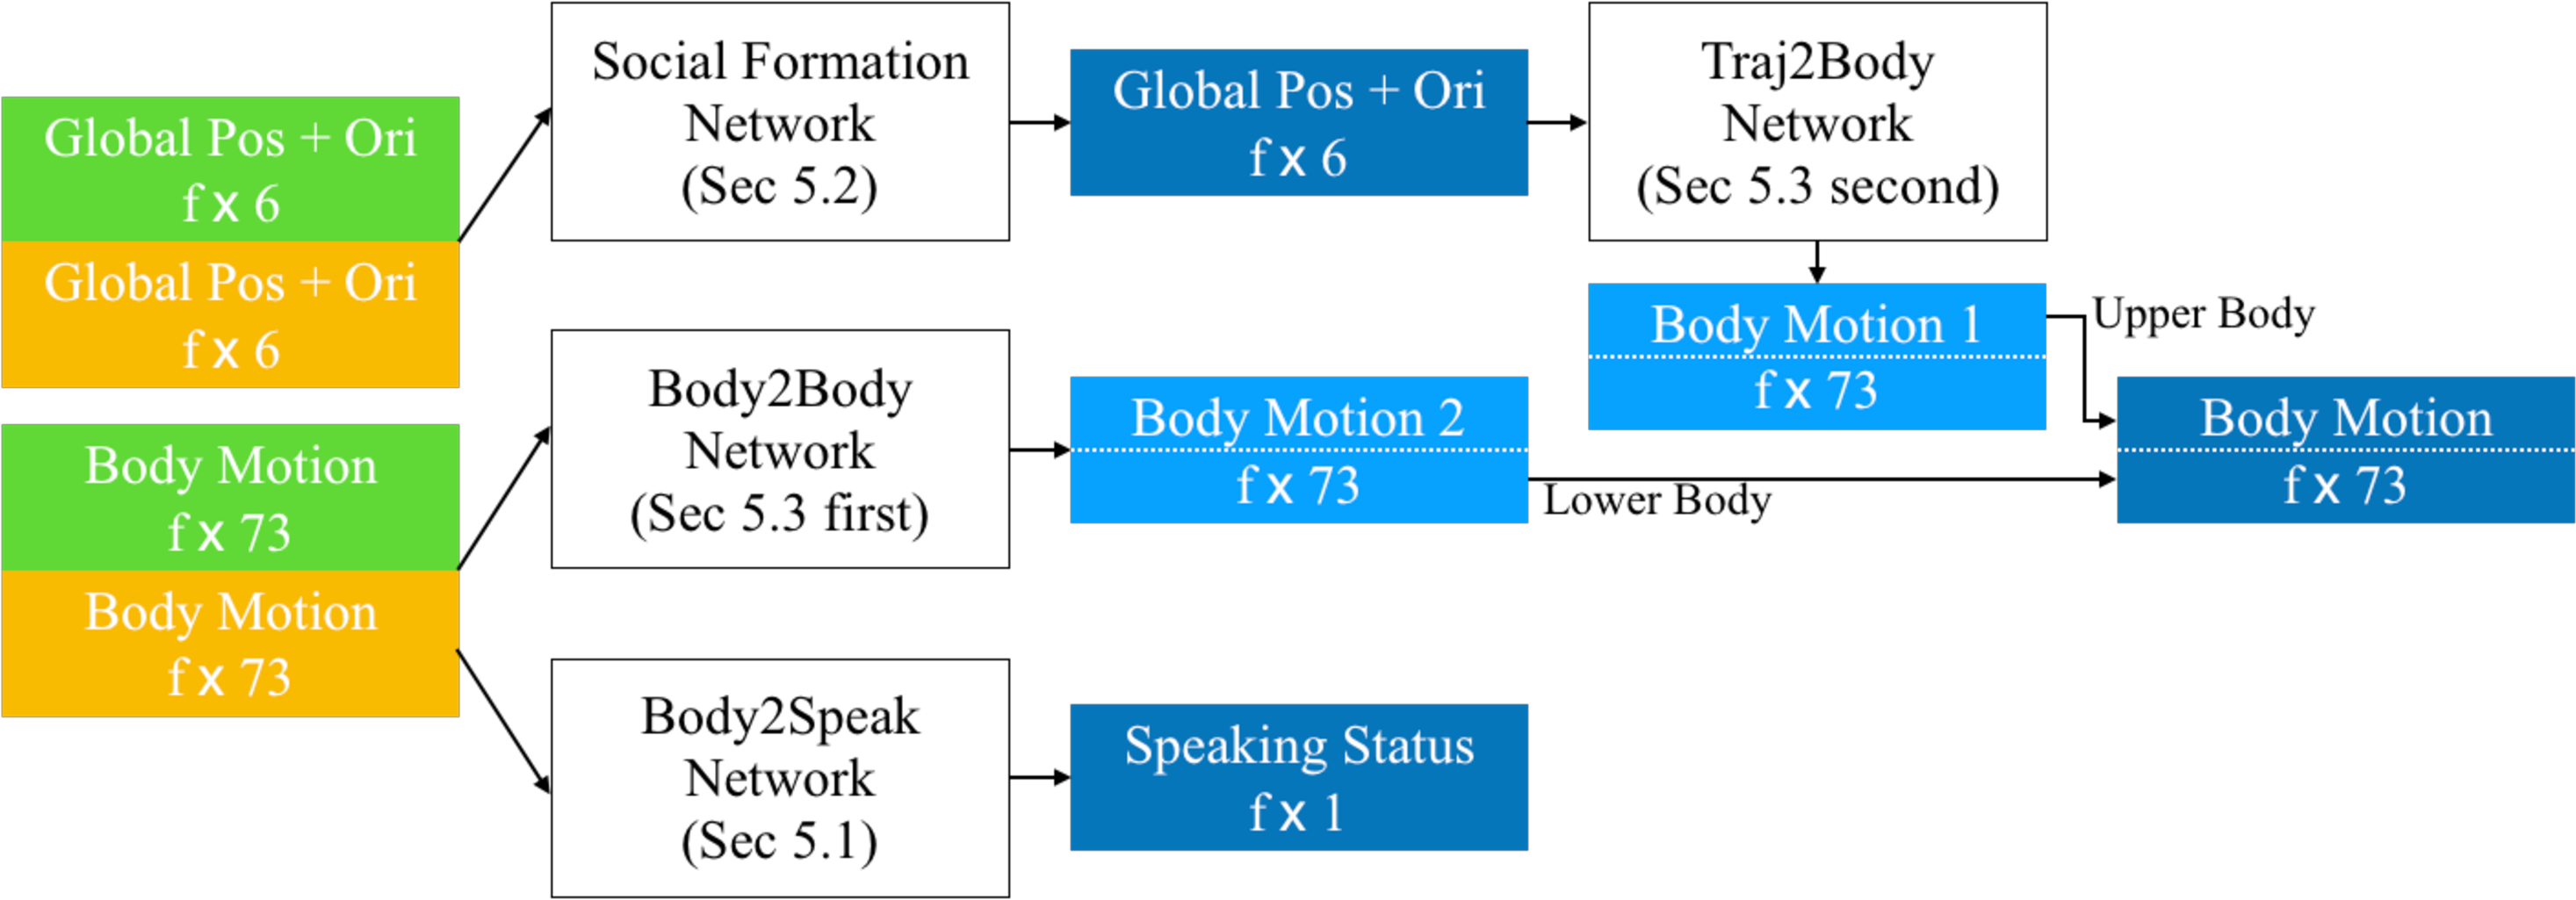
\includegraphics[width=\textwidth]{ssp_fig/ssp_pipeline}
	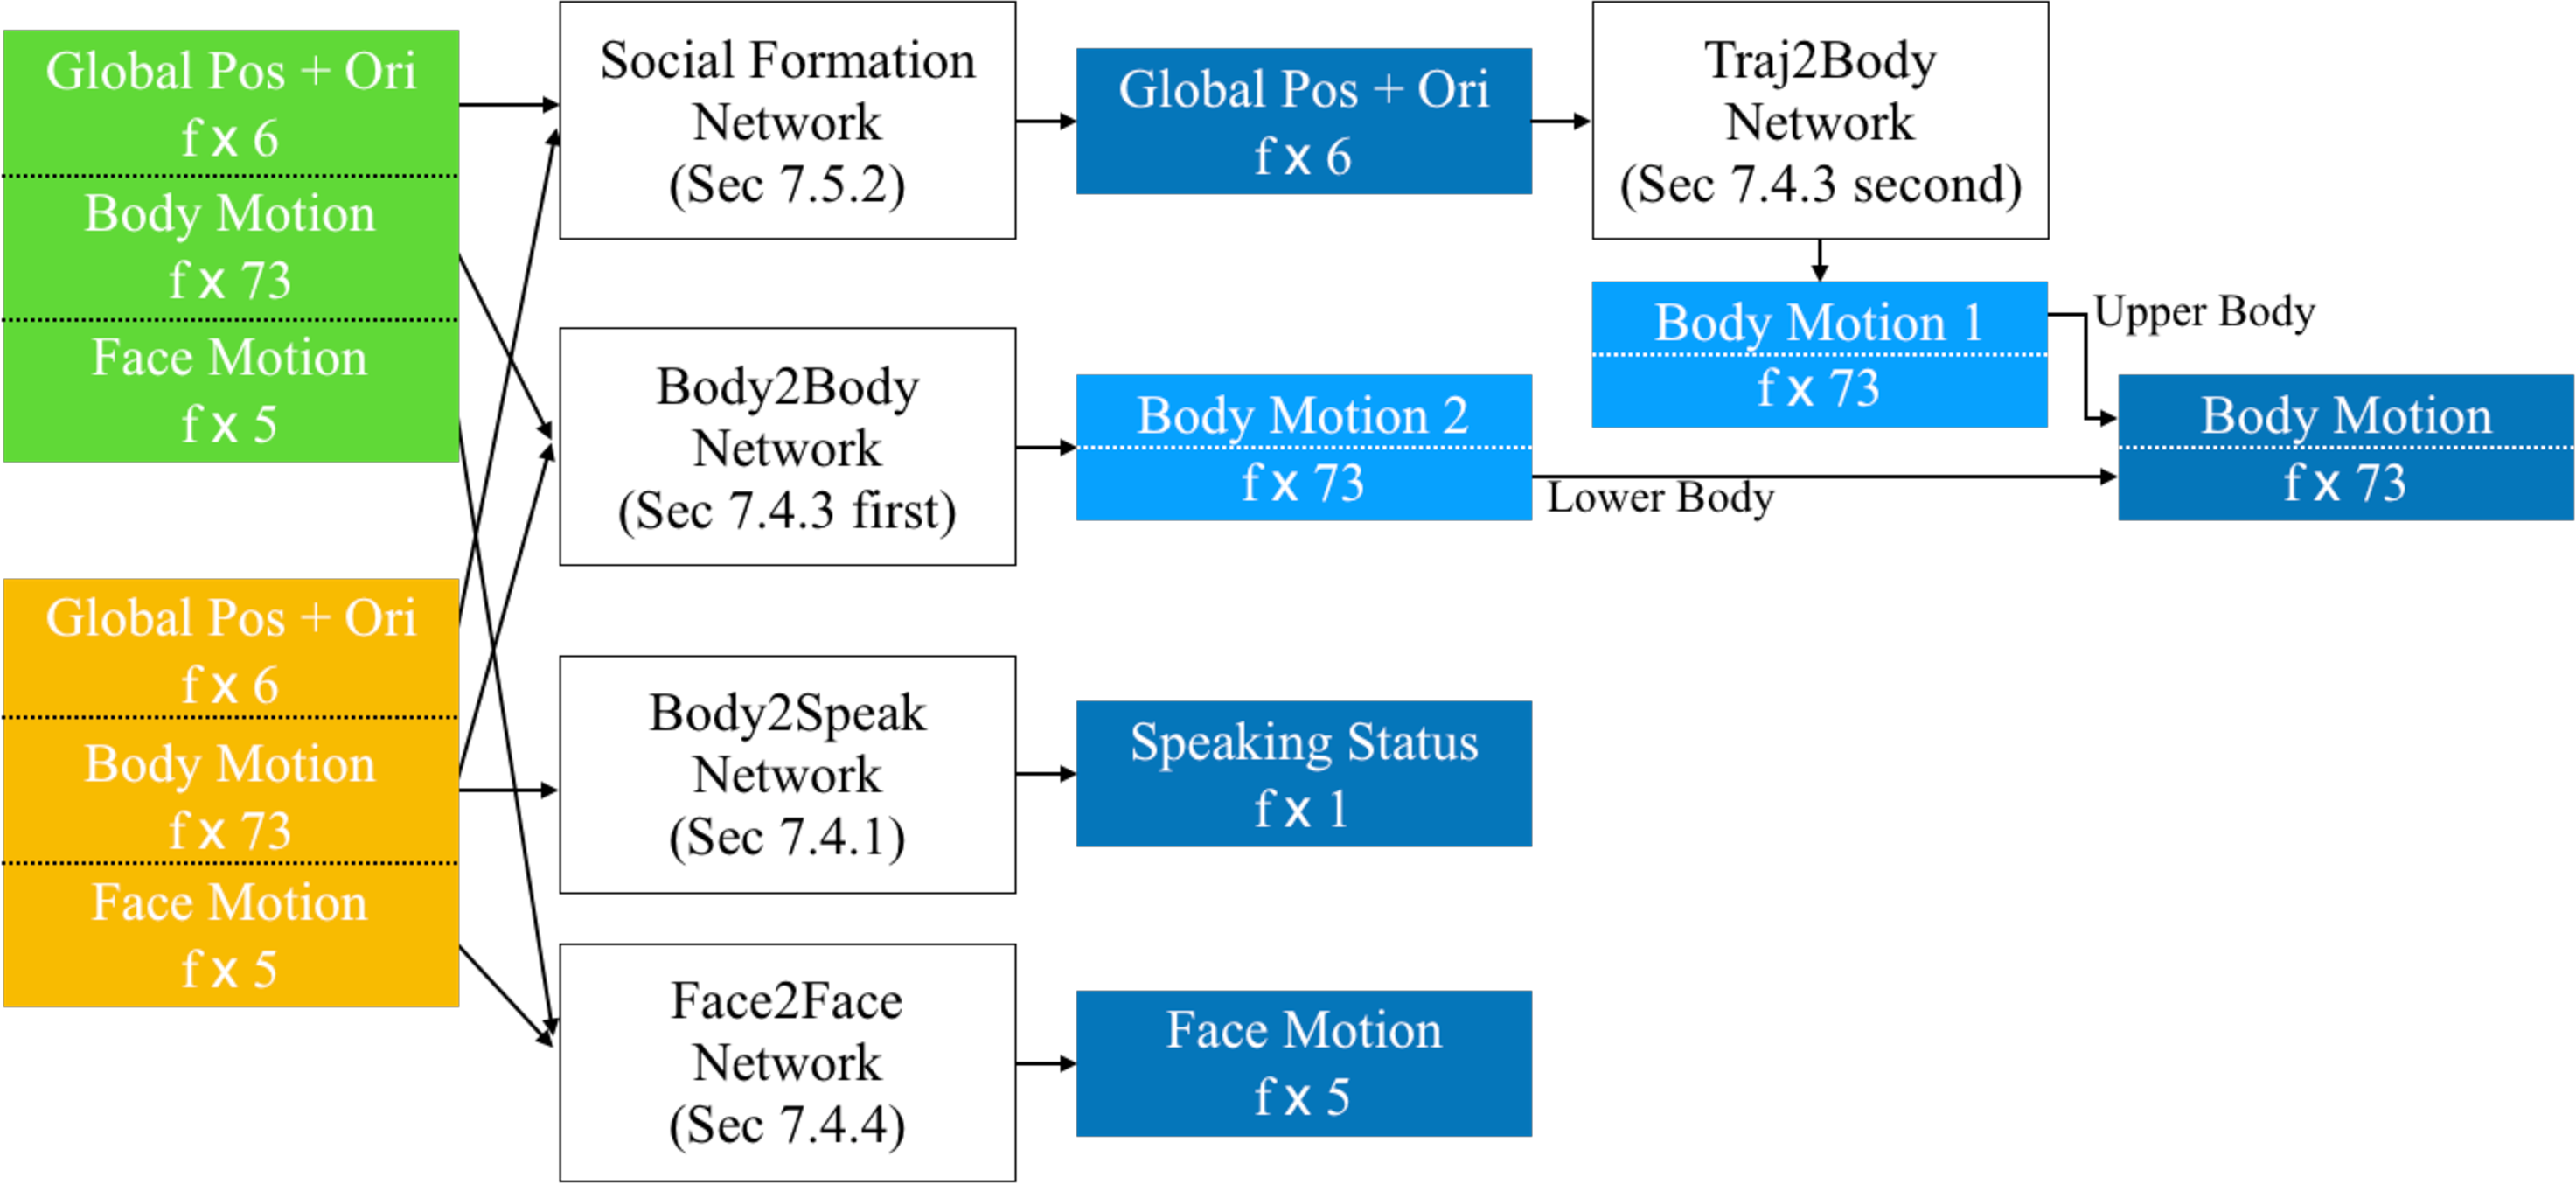
\includegraphics[width=\textwidth]{ssp_fig/ssp_pipeline_wFace}
	\caption{Our Social Signal Prediction Pipeline. We present a baseline method to predict position, orientations, and body gestures, and speaking status of the target subject. }
	\label{fig:pipeline}
\end{figure*}

\subsection{Autoencoder to learn body motion manifold}
\label{sec:autoencoder}
As a preprocessing for body gesture prediction tasks, we first learn the manifold space of the body motion, following the work of \cite{holden2016deep}. We found that this approach is essential to restrict the motion prediction output in a feasible human motion space. We use the same network architecture with \cite{holden2016deep}, using a single convolution layer for each encoder and decoder. The network is shown in the third row of  Figure~\ref{fig:architectures}. The dimension of the latent space is 256 with the half window size of the input, which is larger than the original dimension. Similar to the work of ~\cite{holden2016deep} we add an L1 regularizer in the loss function. After the training, we freeze the decoder part, and use it to decode body motion from the latent code predicted by social prediction tasks.

\subsection{Predicting Body Gestures From A Trajectory (Traj2Body)}
\label{sec:traj2body}
As a baseline method, we regress body motion from the estimated trajectory information of the target person (position and body orientation), as described in Equation~\ref{eq:pred_p2J}. As input, we use the velocities of position and body orientation (relative root movements with respect to the previous frame), which is a part of our body motion representation. For training, we use the ground truth body motion data, where the subpart representing relative root movements as input, and all dimensions of body motion as output. During the testing, we convert the social formation prediction output (global position and orientation) into this velocity representation (relative position and orientation), and use it as the input for our prediction network. The network architecture is shown in the fourth row of Figure~\ref{fig:architectures}. The network predicts the latent code in the body motion manifold space from the 2D trajectory input, and final motion is generated by using a freeze decoder from subsection~\ref{sec:autoencoder}. Note that the decoder is fixed in both training and testing. 

\subsection{Predicting Body Gestures from Other Body Gestures (Body2Body)}

In this case, we use the other two partners' body motions as input. Different from the ``Traj2Body" network in the subsection \ref{sec:traj2body}, we use smaller filter sizes, because we empirically found it makes the body motions more diverse. The network is shown in the fifth row of Figure~\ref{fig:architectures}.

\subsection{Predicting Face Signals from Other Face Signals (Face2Face)}

We use a similar framework with body gesture prediction by learning a manifold space via an autoencoder and predicting the latent code using a regressor, as shown in the sixth row of Figure~\ref{fig:architectures}.

\section{Pipeline of Our Social Signal method}
Each subtask focuses on predicting a part of social signals of the target subject.  To this end,  the predicted social signals are consolidated together to mimic the target person's social behaviors, responding to behaviors of conversational partners. The figure~\ref{fig:pipeline} shows the illustration of the pipeline, where the dark blue boxes are the final outputs. 
